% TU Delft beamer template
% Author: Erwin Walraven (initial version was created by Maarten Abbink)
% Delft Universiy of Technology

\documentclass[xcolor=dvipsnames,aspectratio=169]{beamer}
\usepackage[english]{babel}
\usepackage{graphicx}
\usepackage{subfig}
\usepackage{amsmath}
\usepackage{amsfonts}
\usepackage{amsthm}

\usepackage{tikz}
\usepackage{pgfplots}
\usetikzlibrary{positioning,backgrounds,fit}
\usetikzlibrary{arrows, arrows.meta, calc, quotes, shapes}
\usetikzlibrary{intersections, pgfplots.fillbetween}
\usetikzlibrary{decorations.pathreplacing}


\usetikzlibrary{pgfplots.groupplots}
\usetikzlibrary{patterns}

%\usefonttheme[onlymath]{serif}

\definecolor{pblue}{rgb}{0.12156863,  0.46666667,  0.70588235}
\definecolor{porange}{rgb}{1.        ,  0.49803922,  0.054901965}
\definecolor{pgreen}{rgb}{0.17254902,  0.62745098,  0.17254902}
\definecolor{pgrey}{rgb}{0.5,0.5,0.5}

\setbeamertemplate{navigation symbols}{} % remove navigation symbols
\mode<presentation>{\usetheme{tud}}

% BIB SETTINGS
\usepackage[backend=bibtex,firstinits=true,maxnames=30,maxcitenames=20,url=false,style=authoryear]{biblatex}
\bibliography{bibfile}
\setlength\bibitemsep{0.3cm} % space between entries in the reference list
\renewcommand{\bibfont}{\normalfont\scriptsize}
\setbeamerfont{footnote}{size=\tiny}
\renewcommand{\cite}[1]{\footnote<.->[frame]{\fullcite{#1}}}


\title[]{Data-Driven and Modular Control \\ for Controlled Environment 
Agriculture}
\institute[]{\includegraphics[width=3cm]{TUDelft_logo_rgb.png} \\ Delft Center 
for Systems and Control (DCSC)}
\author{Robert D. (Koty) McAllister}
\date{Bayer Digital Ag Day \\ April 18, 2023}

\begin{document}
{
\setbeamertemplate{footline}{\usebeamertemplate*{minimal footline}}
\frame{\titlepage}
}

{\setbeamertemplate{footline}{\usebeamertemplate*{minimal footline}}

}

\begin{frame}{My background: Optimal control of plants}

\centering
\begin{tikzpicture}[font=\normalsize]
	
	\only<2->{
	\node[align=center,name=atext] at (0,0) {Chemical \\ reactions \medskip \\ 
	Vapor-liquid \\ equilibrium};
	\node[align=center,name=apic] at (2.8,0) 
	{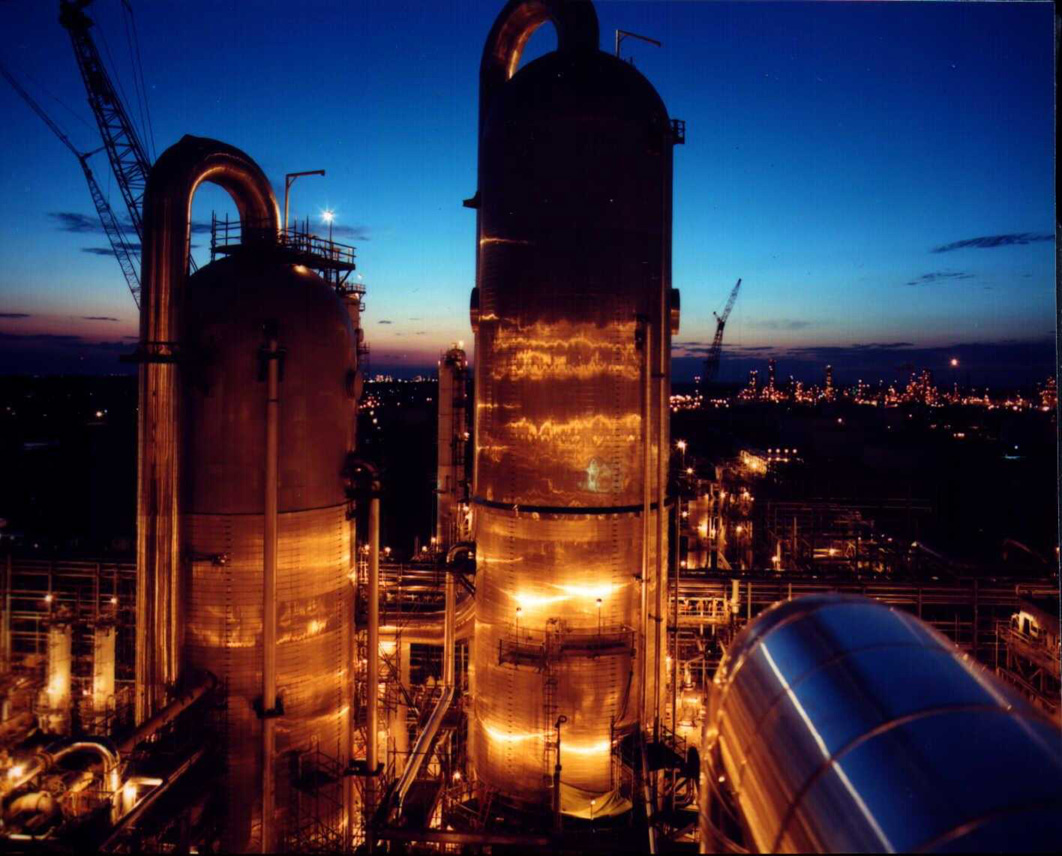
\includegraphics[width=0.21\linewidth]{BasfNightshot.jpg}};
	\node[align=center,name=middle] at (5.9,0) {Economic \\ optimization 
	\medskip \\ Heat \& mass \\ transport};
	\scoped[on background layer]{\node [fit=(atext)(apic)(middle), rounded 
	corners=10mm,draw=porange,fill=porange!30,opacity=0.5,line width= 2pt] {};}
	}
	\only<3->{
		\node[align=center,name=bpic] at (9,0) 
		{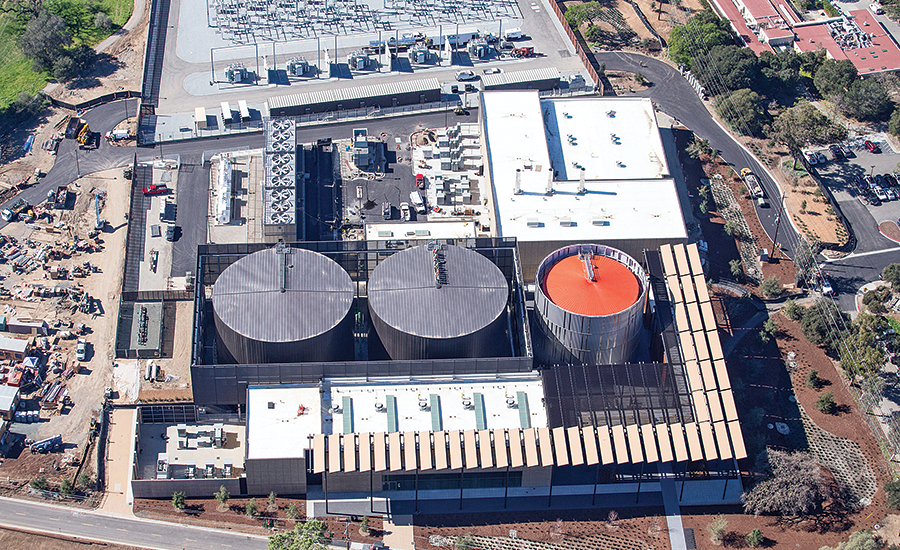
\includegraphics[width=0.21\linewidth]{Johnson_controls_ENRready.png}};
		\node[align=center,name=bpic,opacity=0] at (9,0) {
			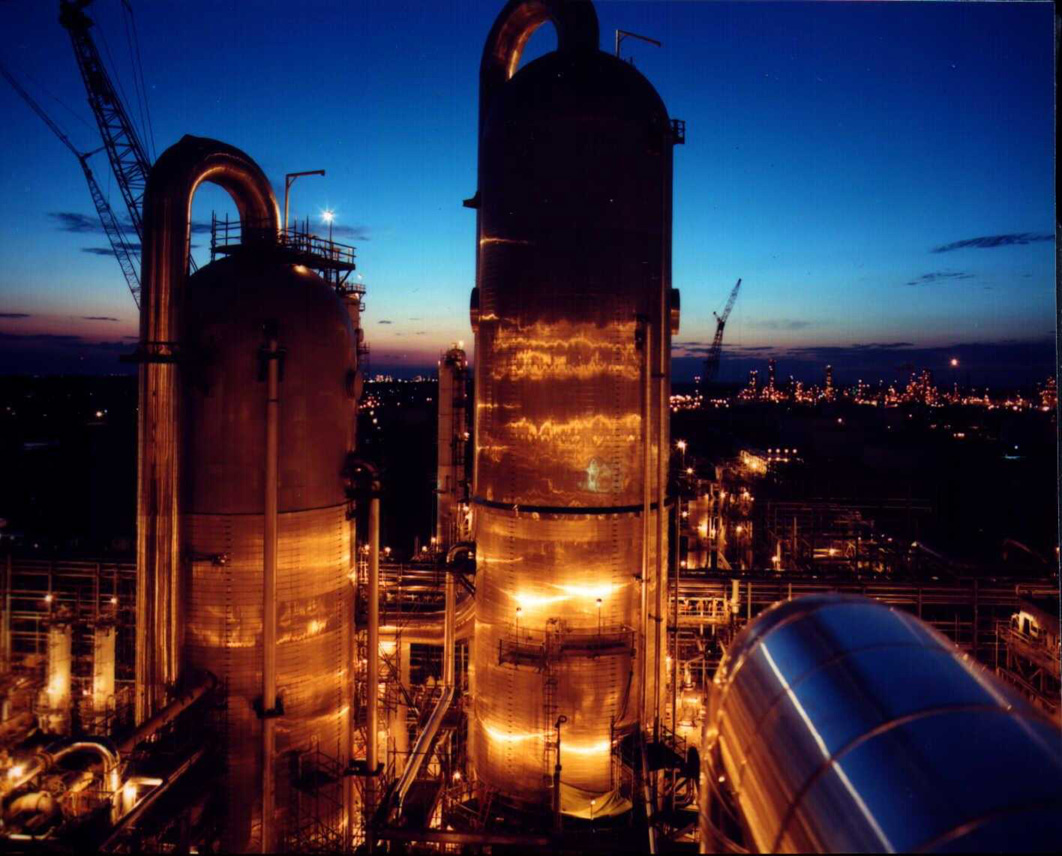
\includegraphics[width=0.21\linewidth]{BasfNightshot.jpg}};
		\node[align=center,name=btext] at (11.8,0) {Time-varying \\ systems 
		\medskip \\ Weather-based \\ disturbances};
		\scoped[on background layer]{\node [fit=(btext)(bpic)(middle), rounded 
		corners=10mm,draw=pblue,fill=pblue!30,opacity=0.5,line width= 2pt] {};}
	}
	
	\scoped[on background layer]{\draw [ rounded 
	corners=10mm,draw=pgreen,fill=pgreen!30,opacity=0,line width= 2pt] 
	(-1.4,-4.5) rectangle (13.4,1.8);}
	\only<4->{
		\node[align=center,name=c] at (5.9,-3) 
		{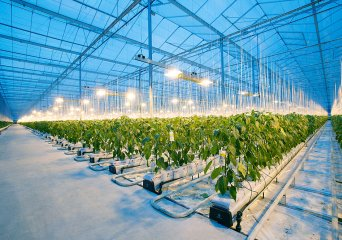
\includegraphics[width=0.25\linewidth]{greenhouse.jpg}};
		\node[align=center] at (1.9,-3) {Biological \\ systems};
		\node[align=center] at (9.9,-3) {Time-scale \\ separation};
		\scoped[on background layer]{\draw [ rounded 
		corners=10mm,draw=pgreen,fill=pgreen!30,opacity=0.5,line width= 2pt] 
		(-1.4,-4.5) rectangle (13.4,1.8);}
	}
\end{tikzpicture}

\end{frame}

\begin{frame}{Controlled environment agriculture (CEA)}
	
	\vspace{0.5cm}
	
	\centering
	\begin{tikzpicture}
	\node[align=center] at (0.5,5) {Heat/cool \\ Light \\ Dehumidify \\ 
	CO\textsubscript{2} Injection};
	\draw[->,>=stealth,line width=2pt] (2,5) -- (3,5);
	\only<1>{
	\node at (5,5) {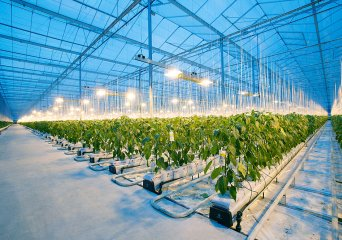
\includegraphics[width=0.25\linewidth]{greenhouse.jpg}};
	}
	\only<2->{
		\node[opacity=0.1] at (5,5) 
		{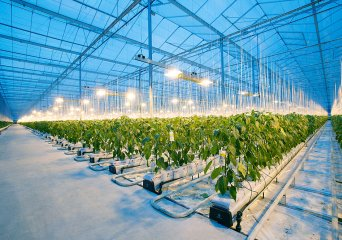
\includegraphics[width=0.25\linewidth]{greenhouse.jpg}};
		\draw[line width=2pt] (3.15,3.7) rectangle (6.85,6.3);
		\node at (5,5) {\Large$x^+ = f(x,u,d)$};
	}
	\draw[->,>=stealth,line width=2pt] (7,5) -- (8,5);
	\node[align=center] at (9.5,5) {T, RH\%, CO\textsubscript{2} \\ Biomass, 
	$\dots$};

	\draw[->,>=stealth,line width=2pt] (2,7.5) -| (5,6.5);
	\node[align=center] {};
	
	\draw [very thick, decorate,decoration={brace,amplitude=8pt}] (1.7,4) -- 
	(-0.7,4) node[align=center,pos=0.5,below=10pt] {\Large $u$};
	\draw [very thick, decorate,decoration={brace,amplitude=8pt}] (10.7,4) -- 
	(8.3,4) node[align=center,pos=0.5,below=10pt] {\Large $x$};
	\draw [very thick, decorate,decoration={brace,amplitude=8pt}] (-1.2,6.5) -- 
	(-1.2,8.5) node[align=center,pos=0.5,left=10pt] {\Large $d$};
	\begin{scope}
		[
		ax/.style={thick, draw=black, cap=rect,line width=1pt},
		xshift=-1cm,
		yshift=6.5cm,
		yscale=0.5,
		xscale=0.5,
		]
		
		\draw[ax,->,>=stealth] (0, 0.2) -- (4.8, 0.2) node[right] {$t$};
		\draw[ax,->,>=stealth] (0, 0.2) -- (0, 4);
		
		\draw [color=pblue,line width=1pt] plot [domain=0:4.3,smooth] 
		(\x,{3.4-0.4*sin(1.5*\x r)});
		\node[color=pblue,right] at (4.3,3.45) {T\textsubscript{a}};
		
		\draw [color=porange,line width=1pt] plot [smooth] 
		coordinates 
		{(1,2) (1.5,2.5) (2,2.6) (2.5,2.8) (3,2.6) (3.5,2)};
		\draw [color=porange,line width=1pt] plot
		coordinates {(0,2) (1,2)};
		\draw [color=porange,line width=1pt] plot
		coordinates {(3.5,2) (4.3,2)};
		\node[color=porange,right] at (4.3,2) {I\textsubscript{a}};
		
		\draw [color=pgreen,line width=1pt] plot [smooth] 
		coordinates 
		{(0,1) (0.5,0.9) (1,1.1) (1.5,1.3) (2,1.4) (2.5,1.4) (3,1.6) (3.5,1.4) 
		(4,1.1) (4.3,1)};
		\node[color=pgreen,right] at (4.3,1) {RH\textsubscript{a}};
	\end{scope}
	
	\end{tikzpicture}

\end{frame}

\newcommand{\greenhouse}[3]{
\draw[line width=1pt] ($ #1 + (0,0) $) rectangle ($ #1 + (#2,#3)$);
\draw[line width=1pt] ($ #1 + (0,#3) $) -- ($ #1 + (0.5*#2,1.25*#3) $);
\draw[line width=1pt] ($ #1 + (#2,#3) $) -- ($ #1 + (0.5*#2,1.25*#3) $);
}

\begin{frame}{Why is the CEA problem so difficult?}
	\centering
	\begin{tikzpicture}[circle dotted/.style={dash pattern=on .05mm off 4mm,
			line cap=round}]
		\greenhouse{(0,0)}{2}{2}
		\draw[->,>=stealth,line width = 2pt] (1,-1) -- (1,0.5);
		\node at (1,-2) {
\includegraphics[width=2cm]{lettuce.png}};
		\onslide<2->{
		\greenhouse{(2.5,0)}{2}{1.2}
		\greenhouse{(5,0)}{1.5}{1.5}
		\draw[->,>=stealth,line width = 2pt] (1,-1) -- (3.5,0.5);
		\draw[->,>=stealth,line width = 2pt] (1,-1) -- (5.75,0.5);
		\draw[line width = 1.5mm,circle dotted] (7.5,1) -- (9,1);
		}
		
		\onslide<3->{
		\node at (3.5,-2) {
\includegraphics[width=2cm]{tomato.png}};
		\node at (6,-2) {
\includegraphics[width=1.5cm]{cucumber.png}};
		
		\draw[line width = 1.5mm,circle dotted] (7.5,-2) -- (9,-2);
		}
	\end{tikzpicture}
	\onslide<4->{
	\begin{block}{}
		\centering
		Many systems with similar physics, but significantly different 
		parameters.
	\end{block} 
	}
\end{frame}

\begin{frame}{A solution: Data-driven and modular controller design}
	
	\vspace{0.3cm} 
	
	\centering
	\begin{tikzpicture}[font=\footnotesize,circle dotted/.style={dash 
	pattern=on .05mm off 4mm,line cap=round}]

		\only<1-3>{
		\draw[line width=2pt,name=sys] (0,0) rectangle (1.5,1) 
		node[align=center, pos=.5] {System 1};
		\draw[line width=2pt,name=data] (2.25,0) rectangle (3.75,1) 
		node[align=center,pos=.5] {Data}; 
		\draw[line width=2pt, ->,>=stealth,color=red] (1.5,2) 
		node[left,align=center] 
		{\textbf{Engineering} \\ \textbf{judgment}} -| (3,1);
		\draw[line width=2pt, ->,>=stealth] (1.5,0.5) -- (2.25,0.5);
		\draw[line width=2pt, ->,>=stealth] (8.25,0.5) -- (9,0.5) 
		node[right] {Deploy!};
		
		\draw[line width=2pt, ->,>=stealth,opacity=0] (1.5,-4) 
		node[left,align=center] 
		{\textbf{Engineering} \\ \textbf{judgment}} -| (3,-3);
		
		}
		
		\only<1-2>{
		\draw[line width=2pt, ->,>=stealth] (3.75,0.5) -- (4.5,0.5);
		\draw[line width=2pt, ->,>=stealth] (6,0.5) -- (6.75,0.5);
		\node[align=center,font=\large] at (-2,-1) {Model-based \\ controller 
			design};
		\draw[line width=2pt] (4.5,0) rectangle (6,1) 
		node[align=center,pos=.5] {Model}; 
		\draw[line width=2pt] (6.75,0) rectangle (8.25,1) 
		node[align=center,pos=.5] {Controller \\ design};
		\draw[line width=2pt, ->,>=stealth,color=red] (2,2) -| (5.25,1);
		\draw[line width=2pt, ->,>=stealth,color=red] (2,2) -| (7.5,1);
		
		}
	
		\only<2>{
		\draw[line width=2pt, ->,>=stealth] (3.75,-2.5) -- (4.5,-2.5);
		\draw[line width=2pt, ->,>=stealth] (6,-2.5) -- (6.75,-2.5);
		\draw[line width=2pt] (4.5,-3) rectangle (6,-2) 
		node[align=center,pos=.5] {Model}; 
		\draw[line width=2pt] (6.75,-3) rectangle (8.25,-2) 
		node[align=center,pos=.5] {Controller \\ design};
		\draw[line width=2pt, ->,>=stealth,color=red] (2,-4) -| (5.25,-3);
		\draw[line width=2pt, ->,>=stealth,color=red] (2,-4) -| (7.5,-3);
		\draw[line width = 1mm,circle dotted] (5.25,-0.5) -- (5.25,-1.5);
		\draw[line width = 1mm,circle dotted] (7.5,-0.5) -- (7.5,-1.5);
		
		}
	
		\only<2-3>{
			
		\draw[line width=2pt,name=sys] (0,-3) rectangle (1.5,-2) 
		node[align=center, pos=.5] {System N};
		\draw[line width=2pt,name=data] (2.25,-3) rectangle (3.75,-2) 
		node[align=center,pos=.5] {Data}; 
		\draw[line width=2pt, ->,>=stealth,color=red] (1.5,-4) 
		node[left,align=center] 
		{\textbf{Engineering} \\ \textbf{judgment}} -| (3,-3);
		\draw[line width=2pt, ->,>=stealth] (1.5,-2.5) -- (2.25,-2.5);
		\draw[line width=2pt, ->,>=stealth] (8.25,-2.5) -- (9,-2.5) 
		node[right] {Deploy!};
		
		\draw[line width = 1mm,circle dotted] (0.75,-0.5) -- (0.75,-1.5);
		\draw[line width = 1mm,circle dotted] (3,-0.5) -- (3,-1.5);
		
		\draw[line width=2pt,rounded corners=10,color=red] (8,-1.5) 
		rectangle (10,-0.5) node[align=center,font=\large] at 
		(9,-1) {\textbf{$\times N$}};
		}
		
		\only<3>{
		\node[align=center,font=\large] at (-2,-1) {\emph{Model-free} \\ 
				controller design};
		\draw[line width=2pt] (4.5, 0) rectangle (8.25, 1) 
		node[align=center,pos=0.5] {\emph{Model-free} controller 
		\\ design (RL, DD-MPC)};
		\draw[line width=2pt, ->,>=stealth] (3.75,0.5) -- (4.5,0.5);
		\draw[line width=2pt, ->,>=stealth,color=red] (2,2) -| (6.325,1);
		
		\draw[line width=2pt] (4.5, -3) rectangle (8.25, -2) 
		node[align=center,pos=0.5] {\emph{Model-free} controller 
			\\ design (RL, DD-MPC)};
		\draw[line width=2pt, ->,>=stealth] (3.75,-2.5) -- (4.5,-2.5);
		\draw[line width=2pt, ->,>=stealth,color=red] (2,-4) -| (6.325,-3);
		\draw[line width = 1mm,circle dotted] (6.325,-0.5) -- (6.325,-1.5);
		
		}
		
		%\draw[dashed] (-0.5,-0.5) -- (11,-0.5);
		
		%\begin{scope}[yshift=-3.2cm]
		\only<4-5>{
			\node[align=center,font=\large] at (-2,-1) {Modular \\ 
			controller design};
			\draw[line width=2pt, ->,>=stealth,color=pblue] (1.5,-3) 
			node[left,align=center] {\textbf{Application}} -| 
			(2.5,-1.5);
			\draw[line width=2pt, ->,>=stealth,color=red] (1.5,1) 
			node[left,align=center] {\textbf{Engineering} \\ 
			\textbf{judgment}} -| (2.5,-0.5);
			\draw[line width=2pt,name=sys] (1,-1.5) rectangle (4,-0.5) 
			node[align=center, pos=.5] {Controller synthesis \\ procedure 
			(CSP)};
			\draw[line width=2pt, ->,>=stealth,opacity=0] (8.25,-2.5) -- 
			(9,-2.5) 
			node[right] {Deploy!};
			
			\draw[line width=1pt, dashed] (4.5,2) -- (4.5,-4);
			
		}
	
		\only<5>{
		\draw[line width=2pt] (5,0) rectangle (6.25,1) 
		node[align=center, pos=.5] {Sys. 1};
		\draw[line width=2pt, ->,>=stealth] (6.25,0.5) -- (7,0.5);
		\draw[line width=2pt] (7,0) rectangle (8.25,1) 
		node[align=center, pos=.5] {CSP};
		\draw[line width=2pt, ->,>=stealth] (8.25,0.5) -- 
		(9,0.5) 
		node[right] {Deploy!};
		
		\draw[line width=2pt] (5,-3) rectangle (6.25,-2) 
		node[align=center, pos=.5] {Sys. N};
		\draw[line width=2pt, ->,>=stealth] (6.25,-2.5) -- (7,-2.5);
		\draw[line width=2pt] (7,-3) rectangle (8.25,-2) 
		node[align=center, pos=.5] {CSP};
		\draw[line width=2pt, ->,>=stealth] (8.25,-2.5) -- 
		(9,-2.5) 
		node[right] {Deploy!};	
		
		\draw[line width = 1mm,circle dotted] (5.625,-0.5) -- (5.625,-1.5);
		\draw[line width = 1mm,circle dotted] (7.625,-0.5) -- (7.625,-1.5);
		
		}
			%\draw[dashed,opacity=0] (-0.5,-0.3) -- (12,-0.3);
		%\end{scope}
	\end{tikzpicture}
	
\end{frame}

\begin{frame}{Applications to CEA: Models}
	\onslide<2->{
	\begin{equation*}
		f(x,u,d) = \color{pgreen}p(x,u,d)\color{black} + 
			\color{porange}g(x,u,d)\color{black}
	\end{equation*}
	}

	\vspace{-0.5cm}
	\onslide<2->{
	\begin{columns}
		\begin{column}{0.45\linewidth}
			\begin{block}{Plant model: $\color{pgreen}p(x,u,d)$}
				\begin{itemize}
					\item High complexity
					\item High data requirements
					\item Centralized
				\end{itemize}
			\end{block}
		\end{column}
		\begin{column}{0.45\linewidth}
			\begin{block}{Greenhouse model: $\color{porange}g(x,u,d)$}
				\begin{itemize}
					\item Low complexity
					\item Moderate data requirements
					\item Local
				\end{itemize}
			\end{block}
		\end{column}
	\end{columns}
	}

	\vspace{0.5cm}
	\centering
	\begin{tikzpicture}[circle dotted/.style={dash pattern=on .05mm off 6mm,
			line cap=round}]
		\greenhouse{(0,0)}{2}{1.5}
		\draw[->,>=stealth,line width = 2pt] (-2,1) -- (0,1);
		\node at (-3,1) {
\includegraphics[width=2cm]{lettuce.png}};
		\draw[->,>=stealth,line width = 2pt] (2,1) -- node[above] 
		{Data} (4,1);
		\draw[line width=2pt] (4,0.5) rectangle (6,1.5) 
		node[align=center, pos=.5] {Sys. ID};
		
		\onslide<-2>{
		\draw[->,>=stealth,line width = 2pt] (6,1) -- (8,1) 
		node[right] 
		{$f(x,u,d)$};
		}
%		\draw[->,>=stealth,line width = 2pt,opacity=0] (-4,1) -- (-5,1) 
%		node[left,color=porange] 
%		{$g_j(\cdot)$};
		
		\onslide<3->{
		\draw[->,>=stealth,line width = 2pt] (6,1) -- (8,1) 
			node[right,color=porange] 
			{$g(x,u,d)$};
		\draw[->,>=stealth,line width = 2pt] (-2,2.3) -| (5,1.5);
		\draw[line width = 2pt] (-3,2) |- (-1,2.3);
		\node[color=pgreen] at (1,2.6) {$p(x,u,d)$};
		}
	\end{tikzpicture}
\end{frame}

\begin{frame}{Optimal control}
	\begin{tikzpicture}[circle dotted/.style={dash pattern=on .05mm off 6mm,
			line cap=round}]
		\begin{axis}
			[
			name = states,
			width = 0.9\textwidth,
			height = 0.5\textheight,
			ymajorticks=false,
			xmajorticks=false,
			axis x line = middle,
			axis y line = middle,
			xmin = 0, xmax = 6.8,
			ymin = 0.05, ymax = 0.8,
			clip = false,
			domain=0:5,
			samples = 6,
			line width=1pt,
			]
			
			\addplot[color=pblue,mark=*,only marks] {0.6 + 0.1*sin(deg(x))}; 
			\addplot[color=pblue,domain=0:5.5,samples=20] {0.6 + 
			0.1*sin(deg(x))}; 
			
			\addplot[color=red,mark=*,const plot] {0.2 + 0.1*cos(deg(x))};
			\addplot[color=red,const plot,domain=5:5.5,samples=2] {0.2 
			+ 0.1*cos(deg(5))};
		
			\draw[line width = 1mm,circle dotted] (axis cs:5.8,0.6) --	(axis 
			cs:6.8,0.6);
			\draw[line width = 1mm,circle dotted] (axis cs:5.8,0.2) --	(axis 
			cs:6.8,0.2);
			
			
			%\addplot[thick, const plot, no marks, porange!50] coordinates 
			%{(0,0.35)};
			
			\node [right, font=\small] at (axis cs: 6.8, 0.05) {$k$};
			\node [align=center, font=\bf, pblue] at (axis cs: -1, 0.55) 
			{State \\ $x$};
			\node [align=center, font=\bf, red] at (axis cs: -1, 0.2) 
				{Input \\ $u$};
			
			\node[align=center] at (axis cs: 0.5,0.86) {$f(x_0,u_0)$};
			\draw[->,>=stealth] (axis cs: 0.05,0.65) to [out=45,in=135] (axis 
			cs: 1,0.72);
			
			\node[align=center] at (axis cs: 1.5,0.9) {$f(x_1,u_1)$};
			\draw[->,>=stealth] (axis cs: 1,0.72) to [out=45,in=135] (axis cs: 
			2,0.72);
			
			\draw[->,>=stealth,opacity=0] (axis cs: 0,0) -- (axis cs: 0,-0.15) 
			node[below] {$\ell(x_0,u_0)$};
			\draw[->,>=stealth,opacity=0] (axis cs: 1,0) -- (axis cs: 1,-0.15) 
			node[below] {$\ell(x_1,u_1)$};
			\draw[->,>=stealth,opacity=0] (axis cs: 2,0) -- (axis cs: 2,-0.15) 
			node[below] {$\ell(x_2,u_2)$};
			
			\only<2->{
			\draw[->,>=stealth] (axis cs: 0,0) -- (axis cs: 0,-0.15) 
			node[below] {$\ell(x_0,u_0)$};
			\draw[->,>=stealth] (axis cs: 1,0) -- (axis cs: 1,-0.15) 
			node[below] {$\ell(x_1,u_1)$};
			\draw[->,>=stealth] (axis cs: 2,0) -- (axis cs: 2,-0.15) 
			node[below] {$\ell(x_2,u_2)$};
			}
			\end{axis}
		\end{tikzpicture}
		
		\onslide<3->{
		\begin{block}{Infinite horizon problem}
		\begin{equation*}
			V_{\infty}(x_0) := \min_{u_0,u_1,\dots} \ \sum_{k=0}^{\infty} 
			\underbrace{\ell(x_k,u_k)}_{\textnormal{Stage Cost}} 
%			\quad 
%			\textnormal{such that } \ \underbrace{x_{k+1} 
%				= f(x_k,u_k)}_{\textnormal{Model}}
		\end{equation*}
		\end{block}
	}
\end{frame}

\begin{frame}{MPC and RL}
	\begin{center}
	Solving the infinite horizon problem is \emph{ideal}, but is typically 
	\emph{intractable}. 
	\end{center}
	
	\bigskip
	
	\begin{columns}
		\pause
		\begin{column}{0.45\linewidth}
			\begin{block}{Model predictive control (MPC)}
				\begin{itemize}
					\item Approximate via finite horizon $N$
					\begin{equation*}
						V_{\infty}(x_0) \approx V_{N}(x_0)
					\end{equation*}
					\item Requires differentiable models
					\item Works well for systems with moderate time-scales
				\end{itemize}
			\end{block}
		\end{column}
		\pause
		\begin{column}{0.45\linewidth}
			\begin{block}{Reinforcement learning (RL)}
				\begin{itemize}
					\item Approximate via parameterization $\theta$
					\begin{equation*}
						V_{\infty}(x_0) \approx \tilde{V}(x_0;\theta)
					\end{equation*}
					\item Allows for ``black-box'' systems
					\item Works well for system with longer time-scales
				\end{itemize}
			\end{block}
		\end{column}
	\end{columns}
\end{frame}

\begin{frame}{A natural hierarchy for plants}
	\centering
	\begin{columns}
		\begin{column}{0.48\linewidth}
			\centering
			\begin{tikzpicture}
				\draw[->,line width=2pt,>=stealth] (4,5) -- (4,4.5);
				\draw[->,line width=2pt,>=stealth] (1,4.5) -- (1,5);
				\draw[->,line width=2pt,>=stealth] (4,3.5) -- (4,3);
				\draw[->,line width=2pt,>=stealth] (1,3) -- (1,3.5);
				\draw[->,line width=2pt,>=stealth] (1.25,0.75) -| (0.5,2);
				\draw[->,line width=2pt,>=stealth] (4.5,2) |- (3.75,0.75);
				\node[align=center] at 
				(2.5,0.75){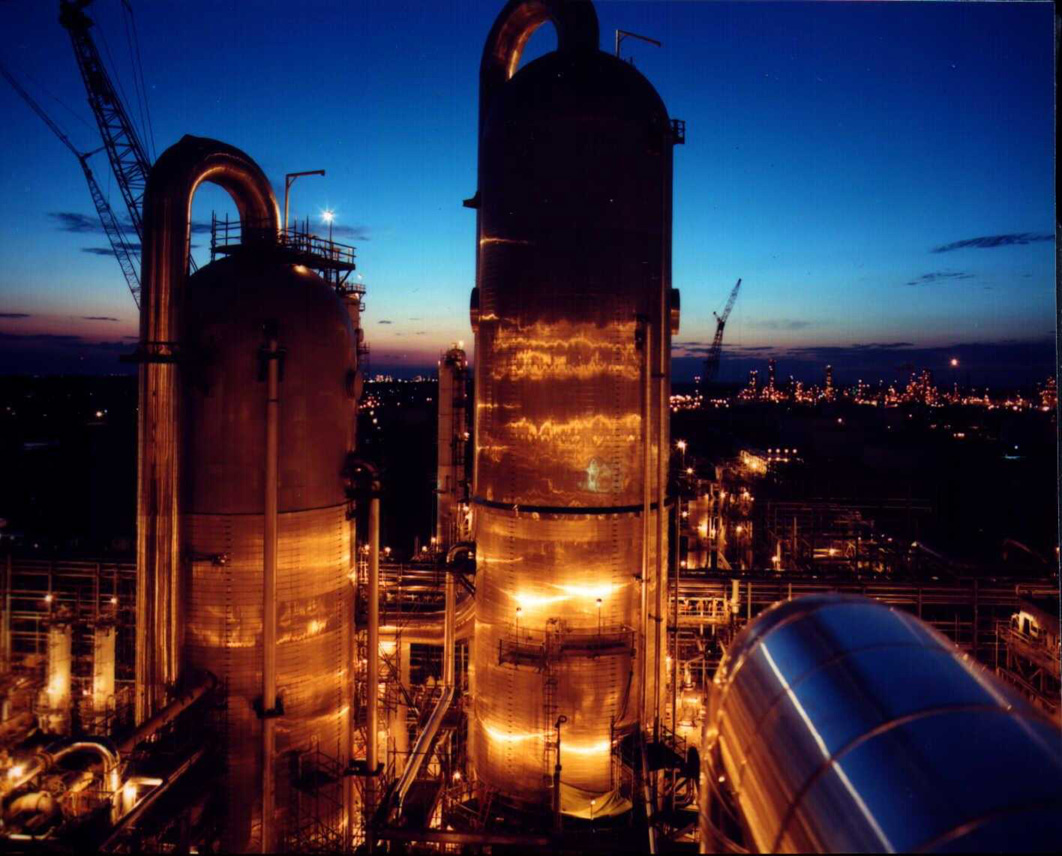
\includegraphics[width=2.5cm]{BasfNightshot.jpg}};
				
				\onslide<-2>{
					\draw[line width = 1.6pt,black] (0,5) rectangle (5,6) 
					node[midway,black,align=center] {Setpoint Optimization \\ 
						(hours-days)};
					\draw[line width = 1.6pt] (0,3.5) rectangle (5,4.5)
					node[midway,black,align=center] {Supervisory Control \\ 
						(minutes)};
					\draw[line width = 1.6pt] (0,2) rectangle (5,3)
					node[midway,black,align=center] {Regulatory Control \\ 
						(seconds)};
				}
				
				\onslide<3->{
					\draw[line width = 1.6pt,black] (0,5) rectangle (5,6) 
					node[midway,black,align=center] {Nonlinear 
					Optimization};
					\draw[line width = 1.6pt] (0,3.5) rectangle (5,4.5)
					node[midway,black,align=center] {\emph{Linear}
					MPC};
					\draw[line width = 1.6pt] (0,2) rectangle (5,3)
					node[midway,black,align=center] {PID \& Rules-based};
				}
			\end{tikzpicture}
		\end{column}
		\pause
		\begin{column}{0.48\linewidth}
			\centering
			\begin{tikzpicture}
				\draw[line width = 1.6pt,black] (0,5) rectangle (5,6) 
				node[midway,black,align=center] {Grower 
				\\ 
					(hours-days)};
				\draw[->,line width=2pt,>=stealth] (4,5) -- (4,4.5);
				\draw[->,line width=2pt,>=stealth] (1,4.5) -- (1,5);
				\draw[line width = 1.6pt] (0,3.5) rectangle (5,4.5)
				node[midway,black,align=center] {Climate Computer \\ (minutes)};
				\draw[->,line width=2pt,>=stealth] (4,3.5) -- (4,3);
				\draw[->,line width=2pt,>=stealth] (1,3) -- (1,3.5);
				\draw[line width = 1.6pt] (0,2) rectangle (5,3)
				node[midway,black,align=center] {Regulatory Control \\ 
					(seconds)};
				\draw[->,line width=2pt,>=stealth] (1.25,0.75) -| (0.5,2);
				\draw[->,line width=2pt,>=stealth] (4.5,2) |- (3.75,0.75);
				\node[align=center] at 
				(2.5,0.75){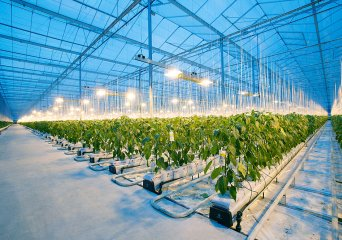
\includegraphics[width=2.5cm]{greenhouse.jpg}};
				\node[align=center,opacity=0] at 
				(2.5,0.75){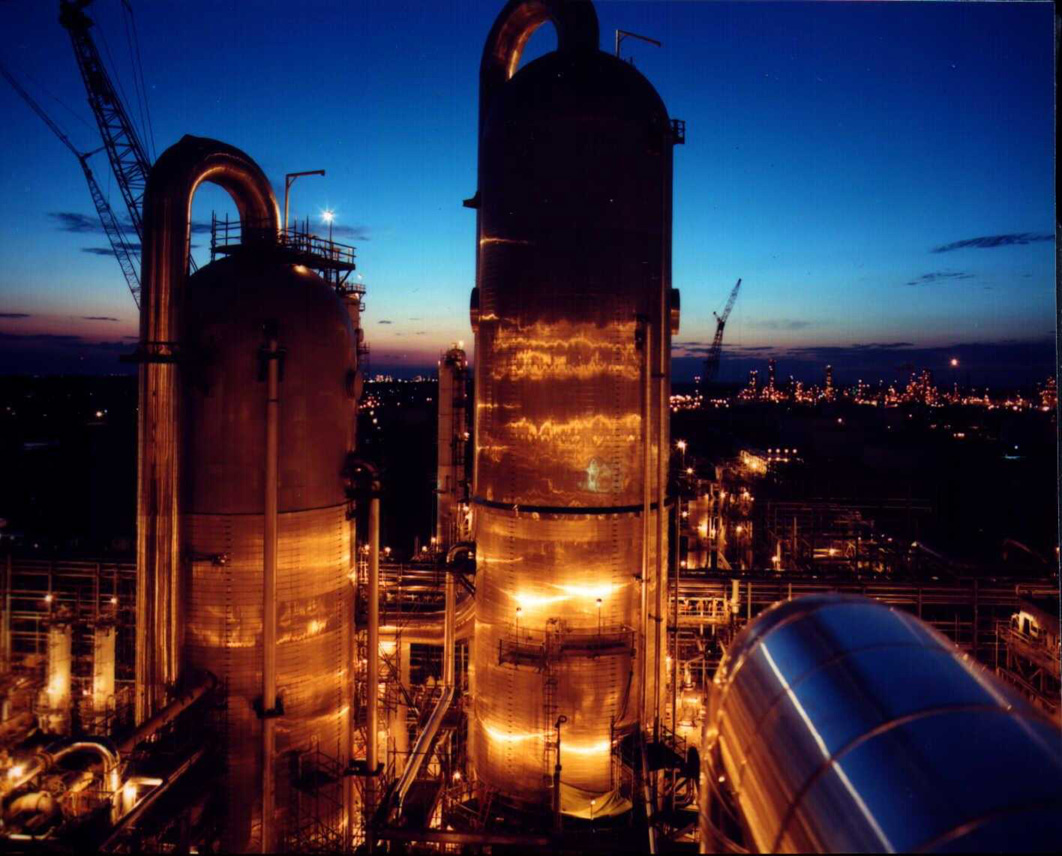
\includegraphics[width=2.5cm]{BasfNightshot.jpg}};
			\end{tikzpicture}
		\end{column}
	\end{columns}
\end{frame}

\begin{frame}{The right tool for every job}
	
	\centering
	\begin{columns}
	\begin{column}{0.48\linewidth}
		\begin{itemize}
			\item Grower: \\ Human $\rightarrow$ RL
			\item Climate Computer: \\ Rule-based $\rightarrow$ 
			MPC
			\onslide<3->{
			\item What should RL and MPC communicate to each other? 
			}
		\end{itemize}
	\end{column}
	
	\begin{column}{0.48\linewidth}
		\centering
			\begin{tikzpicture}
				\draw[->,line width=2pt,>=stealth] (4,5) -- (4,4.5);
				\draw[->,line width=2pt,>=stealth] (1,4.5) -- (1,5);
				\draw[->,line width=2pt,>=stealth] (4,3.5) -- (4,3);
				\draw[->,line width=2pt,>=stealth] (1,3) -- (1,3.5);
				\draw[->,line width=2pt,>=stealth] (1.25,0.75) -| (0.5,2);
				\draw[->,line width=2pt,>=stealth] (4.5,2) |- (3.75,0.75);
				\node[align=center] at 
				(2.5,0.75){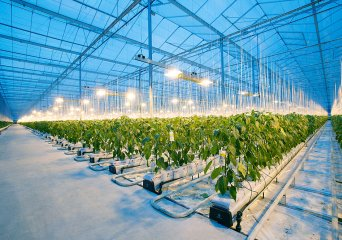
\includegraphics[width=2.5cm]{greenhouse.jpg}};
				\node[align=center,opacity=0] at 
				(2.5,0.75){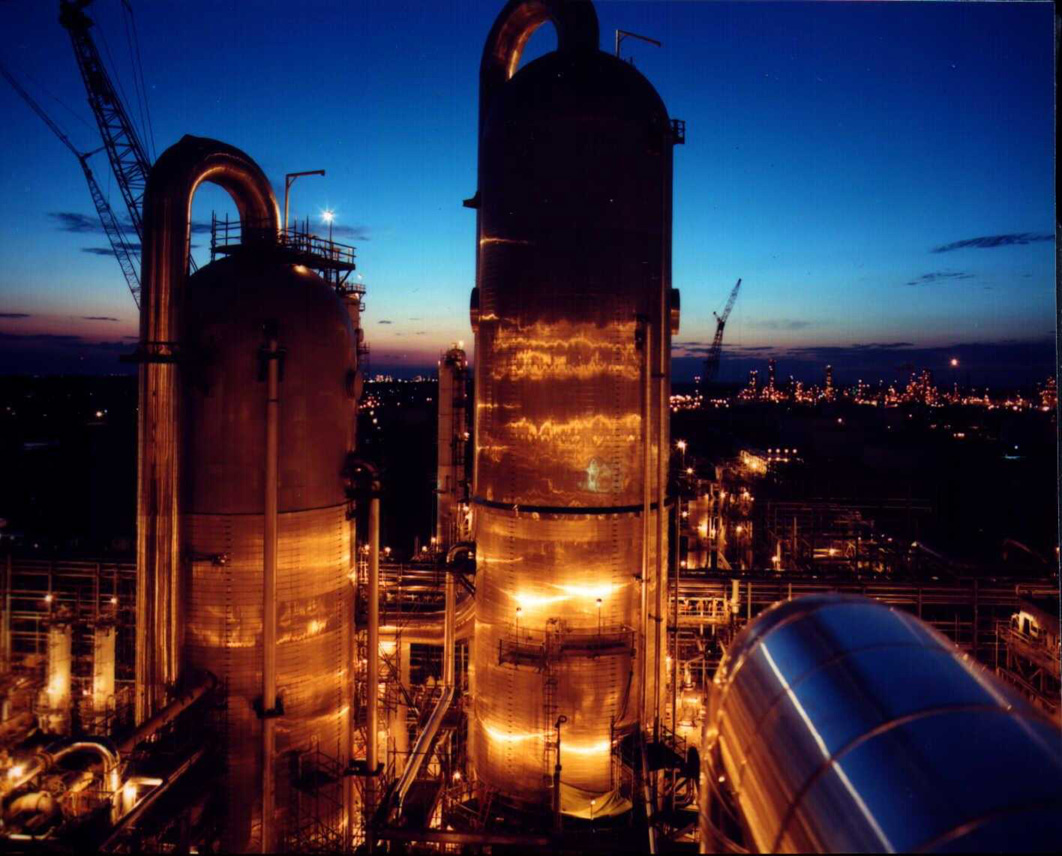
\includegraphics[width=2.5cm]{BasfNightshot.jpg}};
				
				\onslide<1>{
					\draw[line width = 1.6pt,black] (0,5) rectangle (5,6) 
					node[midway,black,align=center] {Grower \\ (hours-days)};
					\draw[line width = 1.6pt] (0,3.5) rectangle (5,4.5)
					node[midway,black,align=center] {Climate Computer \\ 
					(minutes)};
					\draw[line width = 1.6pt] (0,2) rectangle (5,3)
					node[midway,black,align=center] {Regulatory Control \\ 
					(seconds)};
				}
				
				\onslide<2->{
					\draw[line width = 1.6pt,black] (0,5) rectangle (5,6) 
					node[midway,black,align=center] {RL};
					\draw[line width = 1.6pt] (0,3.5) rectangle (5,4.5)
					node[midway,black,align=center] {MPC};
					\draw[line width = 1.6pt] (0,2) rectangle (5,3)
					node[midway,black,align=center] {PID \& Rules-based};
				}
			\end{tikzpicture}
		\end{column}
	\end{columns}
\end{frame}

\begin{frame}{Looking forward: Data-driven and modular controller design}
	\begin{itemize}
		\item Centralized plant models; local greenhouse models
		\pause
		\item RL for high-level, long-term decisions
		\pause
		\item MPC for mid-level, medium-term decisions
		\pause
		\item Research questions:
		\begin{itemize}
			\pause
			\item Algorithms to identify local greenhouse models from data and 
			provided plant model
			\pause
			\item Intelligent communication between RL and MPC layers
			\pause
			\item Including domain knowledge in RL for more data-efficient and 
			explainable results
		\end{itemize}
	\end{itemize}

	\pause
	\bigskip

	\begin{center}
		Thank you for you attention!
		
		\bigskip
		
		Questions and/or comments?
	\end{center}
\end{frame}

\begin{frame}[noframenumbering]{Integrating RL and MPC}
	\begin{enumerate}
		\item Solve for the RL cost $\tilde{V}(x;\theta)$ and higher-level 
		controller with a highly detailed plant model.
		\pause
		\item Use the RL cost in the MPC cost function as a \textit{terminal 
			cost}: 
		\begin{equation*}
			\min_{u_0,\dots,u_{N-1}} \sum_{k=0}^{N-1} \ell(x_k,u_k) + 
			\tilde{V}(x_N;\theta)
		\end{equation*}
		\item Solve the MPC problem with a lower detailed plant model
		\begin{itemize}
			\pause
			\item The MPC controller now sees what the RL controller sees past 
			the horizon $N$. 
			\pause
			\item Solving this optimization problem is typically intractable, 
			but there is a way forward with local approximations!
		\end{itemize} 
	\end{enumerate}
\end{frame}


\begin{frame}[noframenumbering]{RL: How complicated does it need to be?}
	How to best parameterize $\tilde{V}(x;\theta)$?
	\begin{itemize}
		\item The most general, least transparent option: Deep neural networks 
		\begin{equation*}
			\tilde{V}(x;\theta) = h_{NN}(x;\theta) 
		\end{equation*}
		\pause
		\item A more transparent approach that exploits domain knowledge: 
		Basis functions
		\begin{equation*}
			\tilde{V}(x;\theta) = \sum_{i=1}^{n}\theta_i \phi_i(x)
		\end{equation*}
		\begin{itemize}
			\item Choose $\phi_i(x)$ to represent relevant properties, e.g., 
			radiation-to-temperature ratio (RTR), photosynthetic rate, solar 
			daily light integral (DLI), $\dots$ 
			\item Tetris is a classic example of this approach.
		\end{itemize}
	\end{itemize}
\end{frame}

\end{document}
